\documentclass{article}
\usepackage[utf8]{inputenc}
\usepackage{graphicx}
\usepackage{caption}
%\documentclass{minimal}
%\usepackage{amsmath}
\usepackage{array}

\begin{document}

\title{Niesamowity świat liczb pierwszych}
\author{Kerem Özdoğan}
\date{\today}
\maketitle
\section{Wprowadzenie}

\textbf{Liczby pierwsze} to jedne z najbardziej fascynujących elementów matematyki, które intrygują zarówno początkujących, jak i zaawansowanych badaczy.
Te liczby są budulcem wszystkich innych liczb naturalnych, gdyż każdą liczbę można rozłożyć na unikalny zestaw liczb pierwszych. Mimo swojej pozornej prostoty – bycie podzielnym tylko przez 1 i przez siebie – liczby pierwsze skrywają wiele tajemnic. Na przykład ich rozkład w zbiorze liczb naturalnych jest nieprzewidywalny i nie podąża za żadnym oczywistym wzorcem. Dzięki swojej unikalności, liczby pierwsze znalazły zastosowanie w kryptografii, gdzie stanowią podstawę bezpieczeństwa internetowego. Fascynacja nimi rośnie, ponieważ każda nowa odkryta liczba pierwsza przybliża nas do głębszego zrozumienia struktury liczb.
\section{Jakie warunki musi spełnić liczba aby została uznana za pierwszą ?}
\begin{itemize}
    \item Jest liczbą naturalną
    \item Dzieli się \textbf{tylko} przez siebie i przez 1
    
\end{itemize}
\textbf{Uwaga!} Liczby 1 i 0 nie są ani pierwsze ani złożone przez ich właściwości nie pozwalające na rozłożenie ich na skończony niemalejący ciąg pewnych liczb pierwszych.\ref{tab:prime_numbers}
\medskip
\begin{table}[h!]
    \centering
    \begin{tabular}{|c|c|}
        \hline
        \( n \) & \( n \)-ta liczba pierwsza \\
        \hline
        1 & 2 \\
        2 & 3 \\
        3 & 5 \\
        4 & 7 \\
        5 & 11 \\
        6 & 13 \\
        7 & 17 \\
        8 & 19 \\
        9 & 23 \\
        10 & 29 \\
        \hline
    \end{tabular}
    \caption{Tabela 10 początkowych liczb pierwszych}
    \label{tab:prime_numbers}
\end{table}
\end{section}
\medskip
\hfill \break
\medskip
\hfill \break
\medskip
\hfill \break
\medskip
\hfill \break
\medskip
\hfill \break
\medskip
\hfill \break
\section{Optymalny algorytm na sprawdzenie czy liczba jest pierwsza}
Niech liczbą do sprawdzenia będzie liczba n.
\begin{enumerate}
    \item Jeżeli $n<2$ zwróć FAŁSZ
    \item Jeżeli $n==2$ zwróć PRAWDA
    \item Jeżeli n mod 2 == 0 zwróć FAŁSZ
    \item Niech zmienna $i = 3$
    \item Jeżeli $i * i <= n$ idź do kroku nr 6 , w przeciwnym wypadku idź do kroku nr 8
    \item Jeżeli n mod i == 0 zwróć FAŁSZ
    \item Przypisz do wartości zmiennej $i$ wartość $i+2$ i przejdź do kroku nr 5
    \item zwróć PRAWDA
\end{enumerate}
Gdzie a mod b oznacza resztę z dzielnia liczby a przez liczbę b
\section{Próby wzorów na liczby pierwsze}
\begin{equation*}

    \[p_n=1 + \sum_{i=1}^{2^n} \Biggl \lfloor \sqrt[n]{ \Biggl(  \frac{n}{\sum_{j=1}^{i} \lfloor (\frac{cos((j-1)!+1}{j}\pi)^2 \rfloor} \Biggl)}  \Biggr \rfloor \]


    gdzie \lfloor x \rfloor = \max \{ n \in \mathbb{Z} \mid n \leq x \}
\end{equation*}
\medskip
\hfill \break

Wydaje się że skoro istnieje wzór na liczbę pierwszą to cała kryptografia oparta na liczbach pierwszych nie ma sensu. Otóż nie! Wzór podobno działa (sprawdzenie pozostawiam czytelnikowi jako zadanie programistyczne bądź matematyczne), ale ma wadę,suma z sumą w środku powoduje ogromną złożoność jak na taki problem i nie jest zbyt użyteczny lub efektywny.
\section{Piękno liczb pierwszych}
Historia głosi ,że Stanisław Ulam na jednej z konferencji był nudzony, że zaczął \textit{"bazgrolić"} na kartce papieru. Aby zająć sobie głowę zaczął pisać liczby od 1 w spirali.

\begin{figure}[htbp]

    \centering
    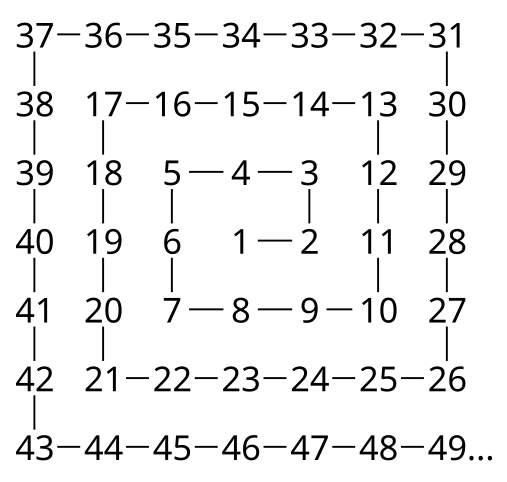
\includegraphics[scale=0.6]{pictures/zdjecia_kerem/u4.png}
    \caption{Odwzorowanie takiej spirali}
    \label{fig:spirala_ulama}
\end{figure}
\medskip
\hfill \break
Po zaznaczeniu liczb pierwszych zobaczymy,że liczby pierwsze "gromadzą" się na ukośnych, można to lepiej zwizualizować większą ilością liczb.
\begin{figure}[htbp]
    \centering
    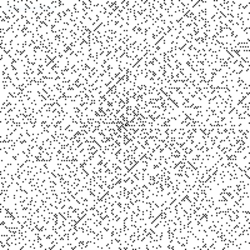
\includegraphics[scale=0.8]{pictures/zdjecia_kerem/u2.png}
    \caption{Odwzorowanie spirali 200 x 200 liczb z liczbami pierwszymi zanzaczonymi jako czarne punkty}
    \centering
    \label{fig:spirala_ulama}
\end{figure}
\medskip
\hfill \break
\section{Klątwa liczb pierwszych}

\textbf{John Nash}, znany ze swoich przełomowych osiągnięć w teorii gier, nie był jedynym matematykiem, który zmagał się z tragicznymi konsekwencjami swojej pasji do liczb pierwszych. "Klątwa liczb pierwszych" odnosi się do niespotykanych nieszczęść, które spotykały wielu badaczy, którzy poświęcali swoje życie tej dziedzinie matematyki. Wśród tych, którzy zmagali się z tragicznymi skutkami, byli matematycy, tacy jak Carl Friedrich Gauss czy Georg Cantor, którzy, w wyniku obsesji na punkcie liczb pierwszych, doświadczali poważnych kryzysów psychicznych, w tym depresji, schizofrenii i paranoi. Ta klątwa stała się niemal legendą w świecie matematyki, sugerując, że dążenie do zrozumienia tajemnic liczb pierwszych może prowadzić do niebezpiecznych konsekwencji.

\textbf{Bernhard Riemann}, badając te zagadnienia, wprowadził hipotezę łączącą rozkład liczb pierwszych z funkcją \textit{zeta Riemanna}. Jego równanie \(\zeta(s) = 0\) dla \(\text{Re}(s) = \frac{1}{2}\) wskazuje na miejsca zerowe, które są kluczowe dla analizy rozmieszczenia liczb pierwszych. Jednak, mimo wielkich osiągnięć, również on nie mógł uciec przed psychologicznymi zmaganiami, które dotykały wielu jego współczesnych. Klątwa ta, związana z tragicznymi losami matematyków, stawia pytanie o cenę, jaką należy zapłacić za próbę zrozumienia tej tajemniczej i frustrującej dziedziny matematyki. Obsesja na punkcie liczb pierwszych może prowadzić do niepewności, a nawet do utraty zdrowia psychicznego, co sprawia, że temat ten pozostaje nie tylko fascynujący, ale także przerażający.

\end{document}